\documentclass[a4paper, 12pt]{article}

\usepackage[margin = 1in]{geometry} % for spacing around
\usepackage{graphicx} % for including images in your pdfs
\usepackage{xcolor} % for including colors in your pdf
\usepackage{soul} % for text decoration
\usepackage[utf8]{inputenc} % for encoded text
\usepackage[T1]{fontenc}
\usepackage{setspace} % for setting different line spacings between paragrafs.
\usepackage{enumerate} % for letting us get more detailed enumerate lists
\usepackage{multirow} % to let us combine more rows together
\usepackage{colortbl} % for decorating tables
\usepackage{amsmath} % used for representing more complicated math displays
\usepackage{supertabular}
\usepackage{longtable} % both of these packages are used to making really big tables
\usepackage{wrapfig} % allows us to wrap text around figures
\usepackage{fancyhdr} % for making fancy headers
%\usepackage{bibtex} % for making better bibliographies
\usepackage[pdftex]{hyperref} % for letting us make links
\usepackage{lscape} % Allows us to flip from portrait to landspace
\usepackage{tikz} % for high detailed drawing
\usepackage{multicol} % To put things side by side
\usepackage{rotating} % For rotating objects
% \usepackage{draftwatermark} % For adding watermarks
\usepackage{MnSymbol} % for using multiple symbols
\usepackage{mathtools} % Used for more math symbols
\usepackage{xfrac} % For more complciated fractions and to add derivitives
\usepackage{hyperref} % for hyper links
\usepackage{enumitem} % for better enum lists
\usepackage{tcolorbox} % for adding colored text boxes
\usepackage{bm} % Adding bold text to math inputs
\usepackage{pgfplots} % Used for plotting functions
\usepackage{booktabs} % For better table rules
\usepackage{tabularx} % For adjustable-width tables
\usepackage{eso-pic} % For adding background images
\usepackage{transparent} % For transparency
\usepackage{fontawesome5}
\usepackage{svg}

% Setting up the default image path
\graphicspath{{./Images/}}

% Implementing authro details
\title{}
\author{}
\date{}

% Setting up the fancy page style
\fancypagestyle{customStyle}{
	\lhead{} \chead{} \rhead{}
	\lfoot{
    \href{https://github.com/EmreArapcicUevak/Smart-Attendance-System}{\faGithub \ GitHub} \hspace{0.5cm}
  } \cfoot{\thepage} \rfoot{
    \href{https://trello.com/invite/b/67d55d04d8b354319f1b1db9/ATTI66010e9dfa09b0a174c6bbc4d1da915388F90333/smart-attendance-ius}{Trello 
\includegraphics[height=10pt]{../GlobalImages/trello-logo.pdf}}
  }
	\renewcommand{\headrulewidth}{0pt}
	\renewcommand{\footrulewidth}{1pt}
}
\pagestyle{customStyle}

% Setting up hyperref options
\hypersetup {
	colorlinks = false,
	citecolor = black,
	filecolor = blue,
	linkcolor = blue,
	urlcolor = blue,
	pdftex
}

\tcbset{
	colback=yellow!10, % Background color
	colframe=red!75!black, % Border color
	width=\textwidth, % Full-width box
	boxrule=0.5mm, % Border thickness
	arc=2mm, % Rounded corners
	fonttitle=\bfseries,
	coltitle=black % Title color
}

% Page layout settings
\geometry{top=1in, bottom=1in, left=1in, right=1in}

% Custom commands


\begin{document}
  
  \begin{titlepage}
    \begin{center}
        % University Logo (Optional)
        
\includegraphics[width=0.45\textwidth]{../GlobalImages/Logo.png} % Change filename if needed
        \vspace{1.5cm}

        {\Huge \textbf{Smart Attendance System}}\\
        \vspace{0.5cm}
        {\Large \textbf{Project Specifications}}\\
        
        \vspace{2cm}
        
        {\large \textbf{Subject:} Software Engineering}\\
        
        \vspace{2cm}
        
        \begin{minipage}[t]{0.48\textwidth}
          \textbf{Students:}\\
          {\large Emre Arapčić-Uevak}\\
          {\large Vedad Siljić}\\
          {\large Ismail Dedić}\\
          {\large Amer Jusić}\\
          {\large Faris Hasanbasić}\\
        \end{minipage}
        \hfill
        \begin{minipage}[t]{0.48\textwidth}
          \raggedleft
          \textbf{Professor:} \\
          {\large Mirza Selimović}\\
          
          \vspace{1cm}

          \textbf{Instructor:} \\
          {\large Adin Jahić}\\
        \end{minipage}


        
        \vfill  % Pushes everything to the top, so date stays at bottom
        
        \textbf{\today}  % Automatically adds the current date
        
    \end{center}
  \end{titlepage}

  \pagebreak
  \tableofcontents
  \pagebreak

  \section{Introduction}
    This section covers the overview and both the Use Case Diagram and EERD to expalin the project

    \subsection{Project Overview}
      The Smart Attendance System is a modern, data-driven solution designed to streamline attendance tracking and class management in educational institutions. The project consists of three main components:
      \begin{enumerate}
        \item A Web Application - Provides access to attendance data, dashboards, and administrative controls.
        \item A Backend Server - Handles data storage, API communication, and system logic.
        \item Native Mobile Applications (iOS \& Android) - Enables attendance tracking and real-time access to schedules.
      \end{enumerate}
    
      \noindent At the core of the system is a centralized database (more about that in Section~\ref{sec: EER}) that maintains records of the organization's structure, including staff, students, class schedules, tutorials, and labs.
      The backend APIs serve as the communication bridge between the database and the web and mobile applications, ensuring secure and efficient data exchange. \\

      \subsubsection{Key Functionalities}
      The system is designed with two main user roles: students and staff, each with distinct access levels and interfaces.
      \begin{itemize}
        \item \textbf{Student Dashboard (Web \& Mobile)} \\
        Students have a calendar-based view of their classes, allowing them to track their schedule and attendance. If they miss too many sessions, they receive alerts and can view their attendance history through a GitHub-style activity tracker that provides a visual representation of their participation.
        \item \textbf{Staff Dashboard (Web \& Mobile)} \\
        Staff members can view and manage the classes they are responsible for. Attendance tracking is done exclusively on mobile devices, where students present their ID cards to be scanned via the professor's (or any other staff member responsible for the class and or session) phone camera. The system reads the barcode on the student’s ID card, ensuring quick and accurate attendance recording.
        \item \textbf{Administrative Controls (Web Only)} \\
        Unlike the mobile applications, the web platform includes an admin panel that allows the organization's management to create and manage user accounts, oversee class structures, and make necessary modifications to the system.
      \end{itemize}

    \newpage
  \section{Detailed Explanation}

    \subsection{Extended Entity Relation Diagram} \label{sec: EER}
      An Entity Relation (\emph{ER}) a graphical representation of entities and their relationships to each other within a database. \newline

      An Extended Entity Relation Diagram (\emph{EER}) is an advanced version of the \emph{ER} diagram that includes additional 
      concepts such as subclasses, specialization, generalization, and categories. It provides a more detailed and comprehensive 
      representation of the data model, capturing more complex relationships and constraints within the system. \newline

      \begin{figure}[h]
        \centering
        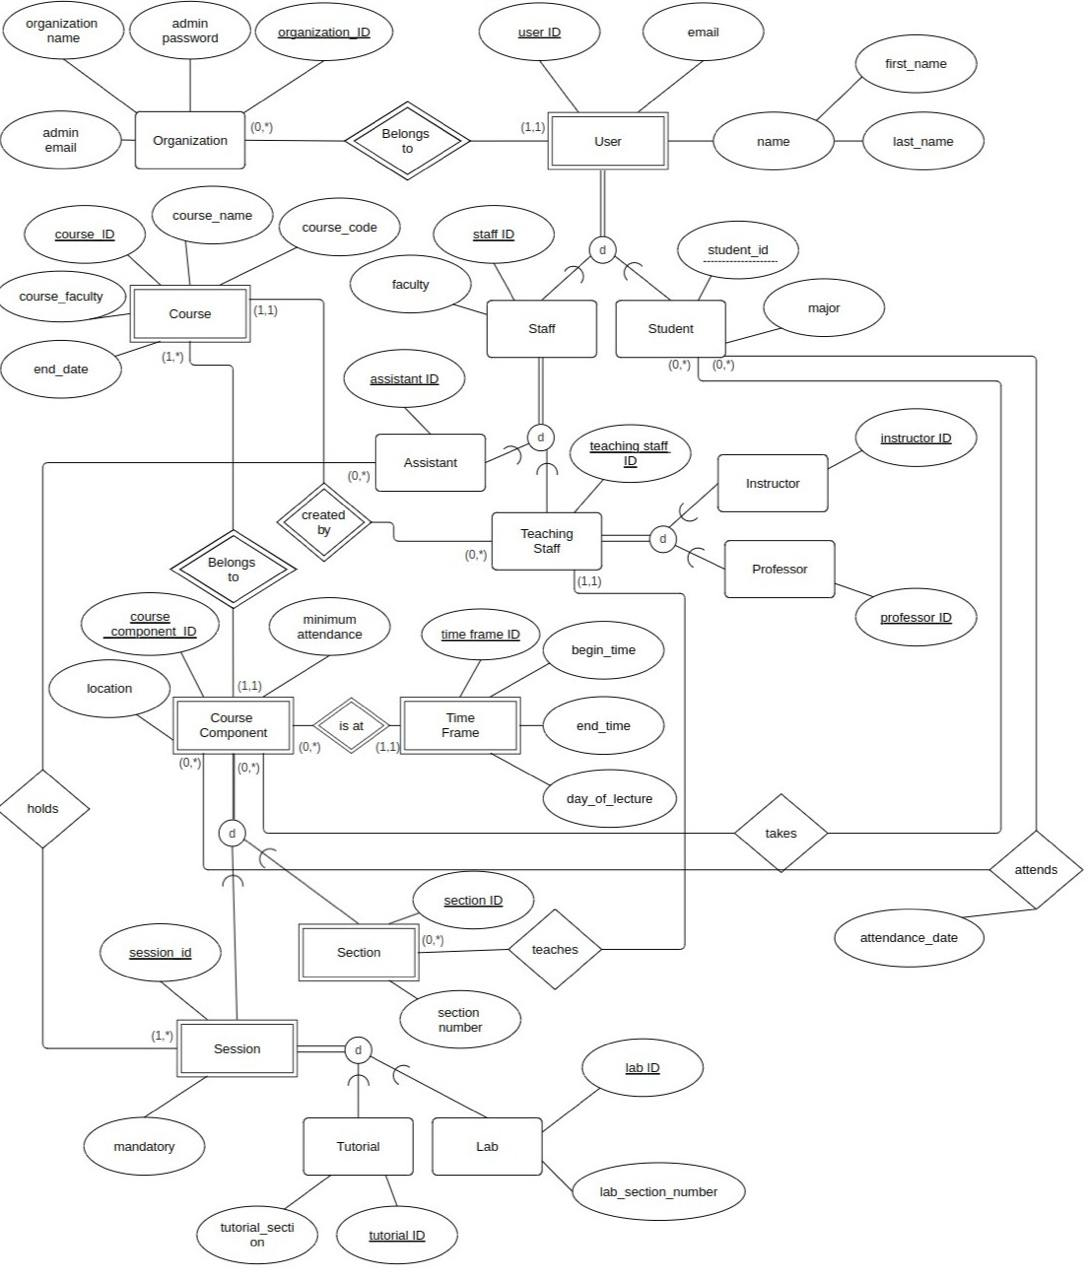
\includegraphics[width=.85\linewidth]{EER_Diagram.jpg}
        \caption{EER Diagram}

        \label{fig:eer-diagram}
      \end{figure}

      \newpage

      \noindent In the figure~\ref{fig:eer-diagram} we can see the EER diagram for our database that we will use as a guide to help us make it.

      \subsubsection{Entities}
        \noindent This section will talk about the entities that can be found in the EER diagram and what they represent
        \vspace{1mm}
        \begin{description}
          \item[Organization] This entity represents the organization, in this case the university, itself which will host all of the users
          \item[User] The User is a \emph{weak entity} of the Organization meaning that's linked to that organization and if that organization ever decides to dissapear all of it's users will not be saved 
          \item[Staff] Staff is a subtype of User which is generally just divided into two more subtypes
          \item[Student] The student in the organization
          \item[Assistant] Staff working in the organization whos job is to hold tutorials
          \item[Teaching Staff] Staff working in the organization whos job is to hold (teach) Course Lectures
          \item[Instructor / Professor] Specializations of the \emph{Teaching Staff} entity
          \item[Course] This entity is the course itself, it is a weak entity of the Teaching Staff entity that created it.
          \item[Course Component] This is a \emph{weak entity} that is used to divide the course into sections for lectures and also \emph{Labs} and \emph{Tutorials}
          \item[Time Frame] This entity tells us more about the course component such as where is it held and during what time.
          \item[Section] This entity represents a section of the course lecture and can be held by other teaching staff
          \item[Session] This is just another subdivison of the course components, it allows for the existence of the \emph{Tutorial} and \emph{Lab} entities that the Assistant needs to teach
          \item [Tutorial / Lab] Specifications of the \emph{Session} entity
        \end{description}
      
      \newpage
      \subsubsection{Relations}
        \noindent This section will talk about the relations that can be found in the EER diagram and what they represent
        \vspace{1mm}

        \begin{description}
          \item[User $\rightarrow$ Organization] belongs to\\
            This is a weak entity saying that an User belongs to only one organization and that an organization can have 0 to many users
          \item[Student $\rightarrow$ Course Component] takes\\
            This relation tells us that a student is partaking in a course component, more generally that a student is currently in "this and that" section of the course
            lecture, tutorial, or lab
          \item[Student $\rightarrow$ Course Component] attends\\
            This relaiton is used to take attendance, and it has its attribute that tells us when the student attended a certain course component
          \item[Asistant $\rightarrow$ Session] holds\\
            This relation tells us which Session (Lab or Tutorial) is held by which Assistant
          \item[Teaching Staff $\rightarrow$ Section] teaches\\
            This relation tells us which Instructor or Professor teaches what section of the course (lecture)
          \item[Course $\rightarrow$ Teaching Staff] created by\\
            This realtion tells us which Instructor or Professor created the course
        \end{description}

        \begin{tcolorbox}[title=Note]
          Please note that we did not include relations for disjoint connections in this list because it does not belong in the scope for the EER.
        \end{tcolorbox}

        \newpage

    \subsection{Use Case Diagram}
\end{document}